\documentclass{article}

\usepackage{ijcai11}
\usepackage{times}
\usepackage{stfloats}
\usepackage{indentfirst}
\usepackage{caption}
\usepackage{subcaption}

\usepackage{graphicx}
\graphicspath{{images}}

\usepackage[hyphens]{url}
\usepackage[colorlinks=true, linkcolor=, urlcolor=blue, citecolor=]{hyperref}
\hypersetup{
	pdfauthor="Aleksandr Sergeev",
	pdftitle="Comparison of neural network and algorithmic based person detectors for LiDAR data"
}

\title{
    Comparison of neural network and algorithmic based person detectors for LiDAR data
}

\author{
    Aleksandr Sergeev \\ 
    Grenoble, France \\
    \href{mailto:aleksandr.sergeev@etu.univ-grenoble-alpes.fr}{\textcolor{black}{aleksandr.sergeev@etu.univ-grenoble-alpes.fr}} \\
    \\
    Supervised by: Olivier Aycard
}

\begin{document}

\maketitle{
    \hbox to0pt{
        \vbox{
            \baselineskip=10dd
            \hrule
            \hbox to\hsize{
                \kern-3pt
                \vrule
                \vbox{
                    \kern3pt
                    \hbox{
                        \small I understand what plagiarism entails and I declare that this report
                    }
                    \hbox{
                        \small is my own, original work.
                    }
                    \hbox{
                        \small Name, date and signature: Aleksandr Sergeev, 21.09.2023.
                    }
                }
                \hfil
                \vrule
            }
            \hrule
        }
    }
}

\parbox[b]{\linewidth}{}

\begin{abstract}
    This paper compares two different methods of detecting people using data from 2D LiDARs, their performance and accuracy are evaluated.
    The "algorithmic detector" is based on an heuristic algorithm, identifying people by detecting clusters of points situated close to each other.
    The "DROW detector" is based on neural network, that used data from the most recent DROW dataset version to fit.
    This network processes five most recent LiDAR measurements and predicts person positions using temporal context.

    The detectors were tested using live data and compared using data from the DROW dataset.
    A special "\texttt{follow\_the\_drow}" library, a Robot Operating System (ROS) package, and a Docker image were introduced for detector comparison and deployment.

    Comparison of precision-recall curves of the detectors revealed that DROW detector is more accurate on DROW dataset.
    However, incorrect annotation issues were found in the dataset, questioning the results.
    In conclusion, although the algorithmic detector has performed better in laboratory, neural network based detectors, that learn from reliably annotated datasets, have greater potential in the real world.
    Future work should focus on reducing the neural network's execution time and dataset annotation accuracy.
\end{abstract}

\section{Introduction}

Light detection and ranging technology (LiDAR) has a wide range of uses in many fields\cite{lidar_market}.
Despite growing availability and active development of 3D LiDARs, 2D LiDARs still remain common in modern robotics\cite{lidar_popularity} and autonomous vehicle industry\cite{lidar_autonomous}.
One of the most challenging tasks in both of the specified fields is person detection.
Not only this task is difficult because people are in many cases very important objects to identify (e.g. autonomous cars), but also because in general human bodies can not be expected to share a common shape in 2D space.

In this work two person detectors of two different types are compared.
One of them uses an heuristic algorithm for determining person positions.
It finds clusters of measure points situated close to each other, clusters of points from 5 to 25 cm in diameter are considered to be "legs".
Similarly, two "legs" not further than 70 cm from each other are considered to be a "person".
This detector will be referenced as "algorithmic detector" later.
The other detector uses a neural network described in "Deep Person Detection in 2D Range Data"\cite{DROW_2018} article and the weights for the network available in the article public GitHub repository\cite{DROW_repo}.
The network consists of 1D convolutional and maxpooling layers.
It processes 5 most recent LiDAR measures simultaneously to make use of the temporal context of detection.
The network returns a vote for every measure point, these votes are converted to predicted person positions later.
This detector will be referenced as "DROW detector" later (just like it was called in the article it originates to).

The robots the detectors were designed for (Karl for DROW detector and RobAIR\cite{RobAIR_site} for algorithmic detector) do not differ much in terms of LiDAR type and positioning.
In both cases 2D LiDARs with similar fields of view were used (225\textdegree{} for Karl and 255\textdegree{} for RobAIR).
In both cases the LiDARs were positioned approximately on knee height (37cm for Karl and around 10cm for RobAIR).
This allowed using the same dataset, originally prepared and annotated for "DROW: Real-Time Deep Learning based Wheelchair Detection in 2D
Range Data"\cite{DROW_2016} article, for detector evaluating and comparing.

\section{Comparison of person detectors}

\begin{figure*}[t!]
	\centering
	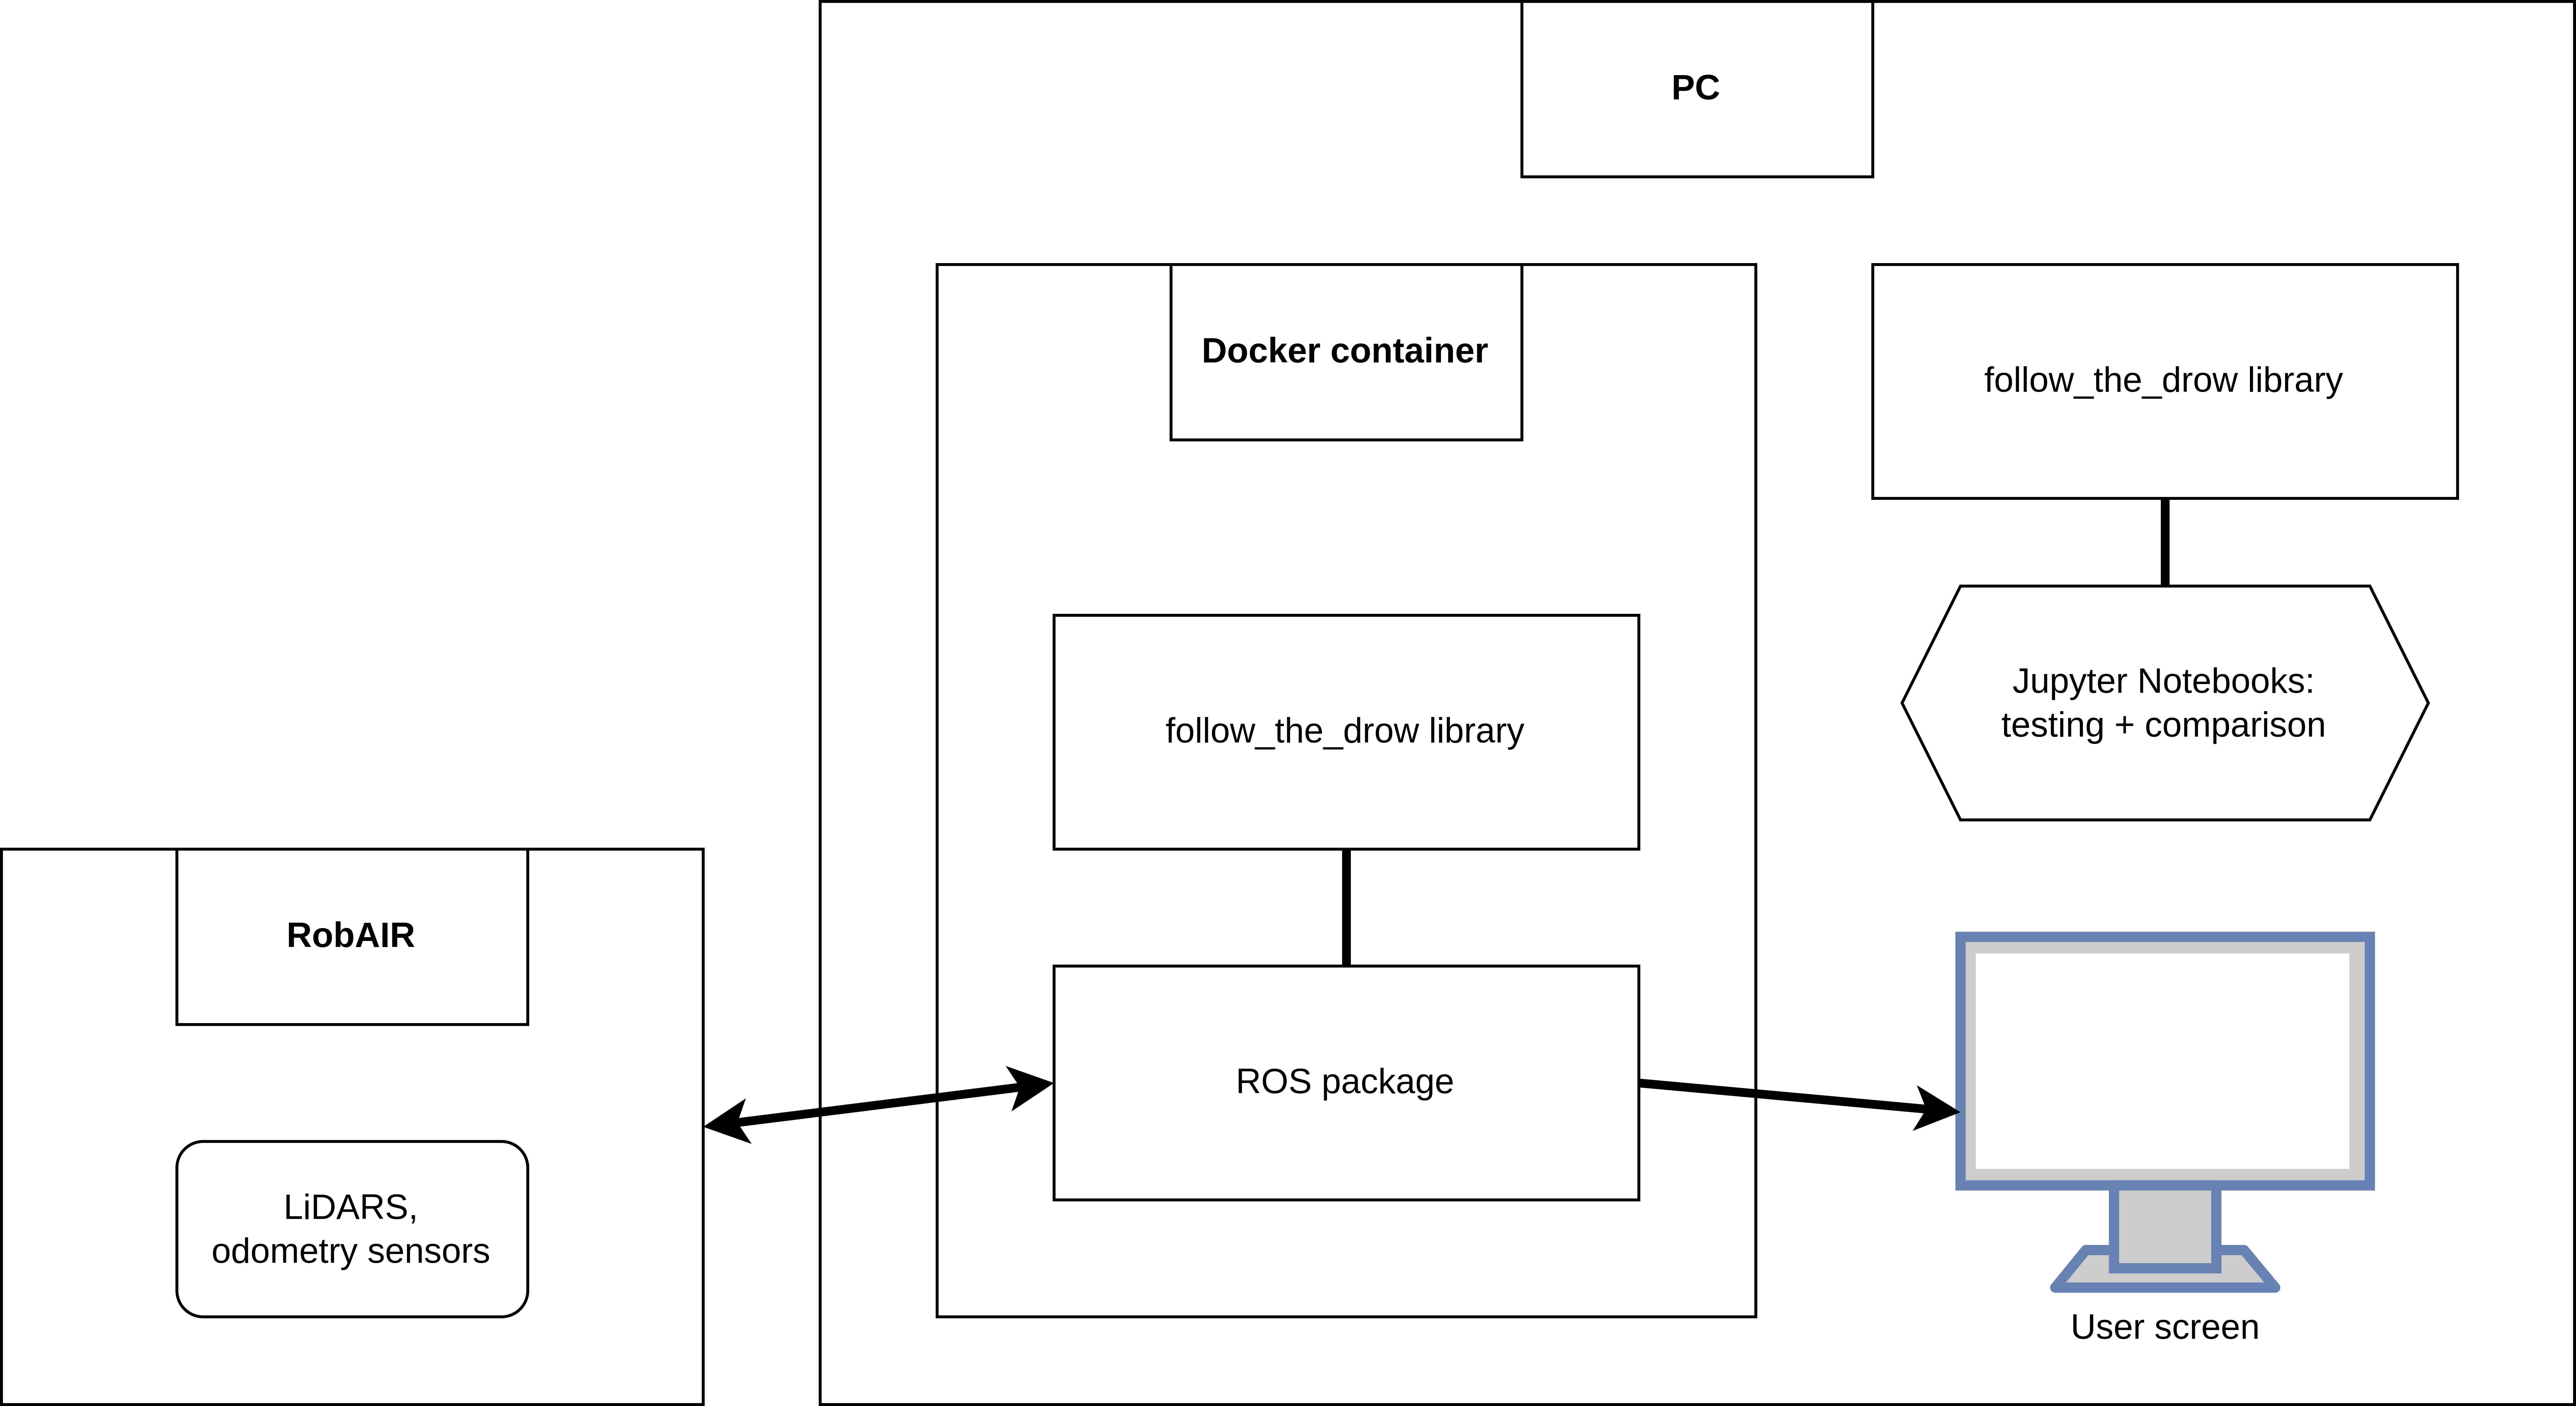
\includegraphics[width=0.9\textwidth]{ftd_setup_chart}
	\caption{Library and package setup chart}
	\label{fig:ftd_setup_chart}
\end{figure*}

Comparison of the algorithmic and DROW detectors requires their execution in the similar environments and on the same input data.
In order to launch both detectors and receive their output, a library with and Python interface for both detectors was written.
For launching the detectors on RobAIR, a Robot Operating System (ROS)\cite{ros_site} package containing LiDAR data collector, transformer and detector nodes was created.
In order to launch the pipeline on machines that do not have ROS installed, a Docker image containing the source code was introduced.

Figure \ref{fig:ftd_setup_chart} shows the setup that was used for detectors execution and comparison.
Detector comparison was performed locally on a laptop using DROW dataset and \texttt{follow\_the\_drow} library.
The results obtained were stored in Jupyter notebooks.
Live detector testing was performed on a laptop connected to a RobAIR.
The \texttt{follow\_the\_drow} ROS package was run locally in Docker container, it used input live data from RobAIR sensors and displayed detection results on screen with RVIZ\cite{rviz_wiki} package.

The \texttt{follow\_the\_drow} library, ROS package and Docker image are considered to be contribution of this work.
All of them can be reused for comparing different person detectors and just running any ROS packages in Docker (with minor changes) with or without connection to a physical robot.

\subsection{\texttt{follow\_the\_drow} library}

The library consists of three parts.

Datasets part contains the dataset described in DROW article together with some useful methods for loading and acquiring data from it.
The second dataset available is the live dataset, that provides similar interface for working with live data received from robot scanners in runtime.

Detector part contains the DROW detector, it is equipped with a few methods for convenient detected person position votes processing.
There also is a \texttt{Python} wrapper for the algorithmic detector that is originally written in \texttt{C++}, the \texttt{C++} code also resides in the library.

The final part is the utilities part, it contains not only utility functions used by the DROW article authors in their public repository, but also some other useful methods for DROW dataset automatic downloading and result caching.

\subsubsection{DROW dataset provider}

The DROW dataset itself is automatically packaged and distributed together with the \texttt{follow\_the\_drow} library.
Dataset provider loads all the data simultaneously into memory and keeps it there.
The dataset contains data from one (knee-height) LiDAR only, so it has only one method for data retrieval, the data received from it should be considered as "bottom".
Since DROW detector processes five latest measures and algorithmic detector processes one detection at a time, the retrieval function combines one or more latest measures into array.

\subsubsection{Live dataset provider}

The live dataset provider emulates dataset for live data.
It accumulates measures in a queue of requested, returns and empties the queue upon data retrieval.
It has support for receiving (and retrieving by detector) data from two LiDARs simultaneously.

\subsubsection{DROW person detector}

DROW person detector is adapted from DROW\cite{DROW_2018} article.
It utilizes a neural network model built with pytorch\cite{pytorch_site} library.
The neural network casts a vote for object location for a fixed-size window around every measure point.
At every time it processes five latest measures in order to keep track of temporal changes in input data.
It is only capable of processing bottom LiDAR measures.
The detector returns arrays of votes and confidencies, that can be later transformed into predicted person positions using library functions.

\subsubsection{Algorithmic person detector}

Algorithmic person detector was adapted from \textbf{Follow me behavior} \cite{follow_me_behavior} article.
It was changed so that it would benefit from using advanced \texttt{C++} features (links, vectors, etc.) and also become configurable at runtime.
The algorithm searches for objects represented by certain patterns of "clusters" of points situated close to each other.
It is capable of processing bottom LiDAR measures (15cm from the ground) only as well as top (1.6m from the ground) and bottom LiDAR measurements together.
The detector returns an array of predicted person positions.

Follow the DROW library also provides a binding of the algorithm \texttt{C++} code to \texttt{Python} class using \texttt{pybind11}\cite{pybind_site} library.

\subsection{Follow the DROW ROS package}

\begin{figure*}[t!]
	\centering
	\includegraphics[width=0.9\textwidth]{ftd_package_chart}
	\caption{Follow the DROW ROS package chart}
	\label{fig:ftd_package_chart}
\end{figure*}

\begin{figure}[b!]
	\centering
	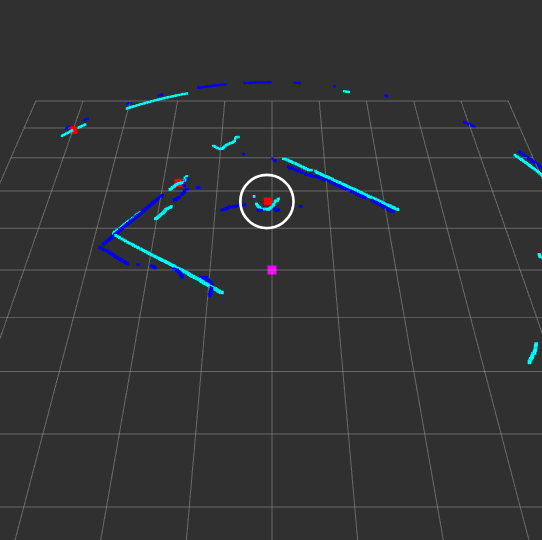
\includegraphics[width=0.75\linewidth]{ftd_live_output}
	\caption{Visualizer node live output}
	\label{fig:visualizer_node_live}
\end{figure}

A ROS package was created for launching the detectors on local machine using input data from real-world (RobAIR) environment.
The package requires follow\_the\_drow library.
Figure \ref{fig:ftd_package_chart} demonstrates nodes of follow the DROW ROS package and topics they read data from and write to.
It contains the following nodes:

\begin{enumerate}
	\item \textbf{Live Loader} loads live data from RobAIR LiDAR(s), input topics are configurable, outputs raw measurements and odometry data.
	\item \textbf{File Loader} loads data from DROW dataset, outputs raw measurements and odometry data.
	\item \textbf{Algorithmic detector} processes data using algorithmic detector and outputs array of person positions.
	\item \textbf{DROW detector} processes data using DROW detector and outputs array of person positions.
	\item \textbf{Person tracker} tracks a single person from arrays outputted by selected detector node, it has several tracking policies.
	\item \textbf{Visualizer} visualizes all data in system (raw measurements data, annotations data, detections data, tracked person position).
	\item \textbf{Annotator} can be used for DROW dataset manual re-annotation, uses RVIZ interface for person position setting.
\end{enumerate}

Properties of physical RobAIR are set up manually as input parameters of the \textbf{Live Loader} node.
The central point of the RobAIR is considered to be the center of its' base on ground level.
The default value for bottom LiDAR offset is 15cm towards positive X (front side of the RobAIR).
The default value for top LiDAR offset is 1.2m towards positive Y (top side of the RobAIR).
The LiDAR offsets can be given both in cartesian and in polar coordinates.

Figure \ref{fig:visualizer_node_live} shows output of the \textbf{Visualizer} node in the ROS package launched on a physical RobAIR inside LIG laboratory.
Pink marker represents RobAIR itself, dark blue markers represent lower LiDAR data, cyan markers represent top LiDAR data and red markers represent algorithmic detector person predictions.
Green markers should represent DROW detector person predictions, but the detector did not find anything.
The closest to the RobAIR prediction is accurate (it is marked with white circle), the others are false positives.

\subsection{Follow the DROW Docker image}

\begin{figure*}[t!]
	\centering
	\begin{subfigure}{.5\textwidth}
		\centering
		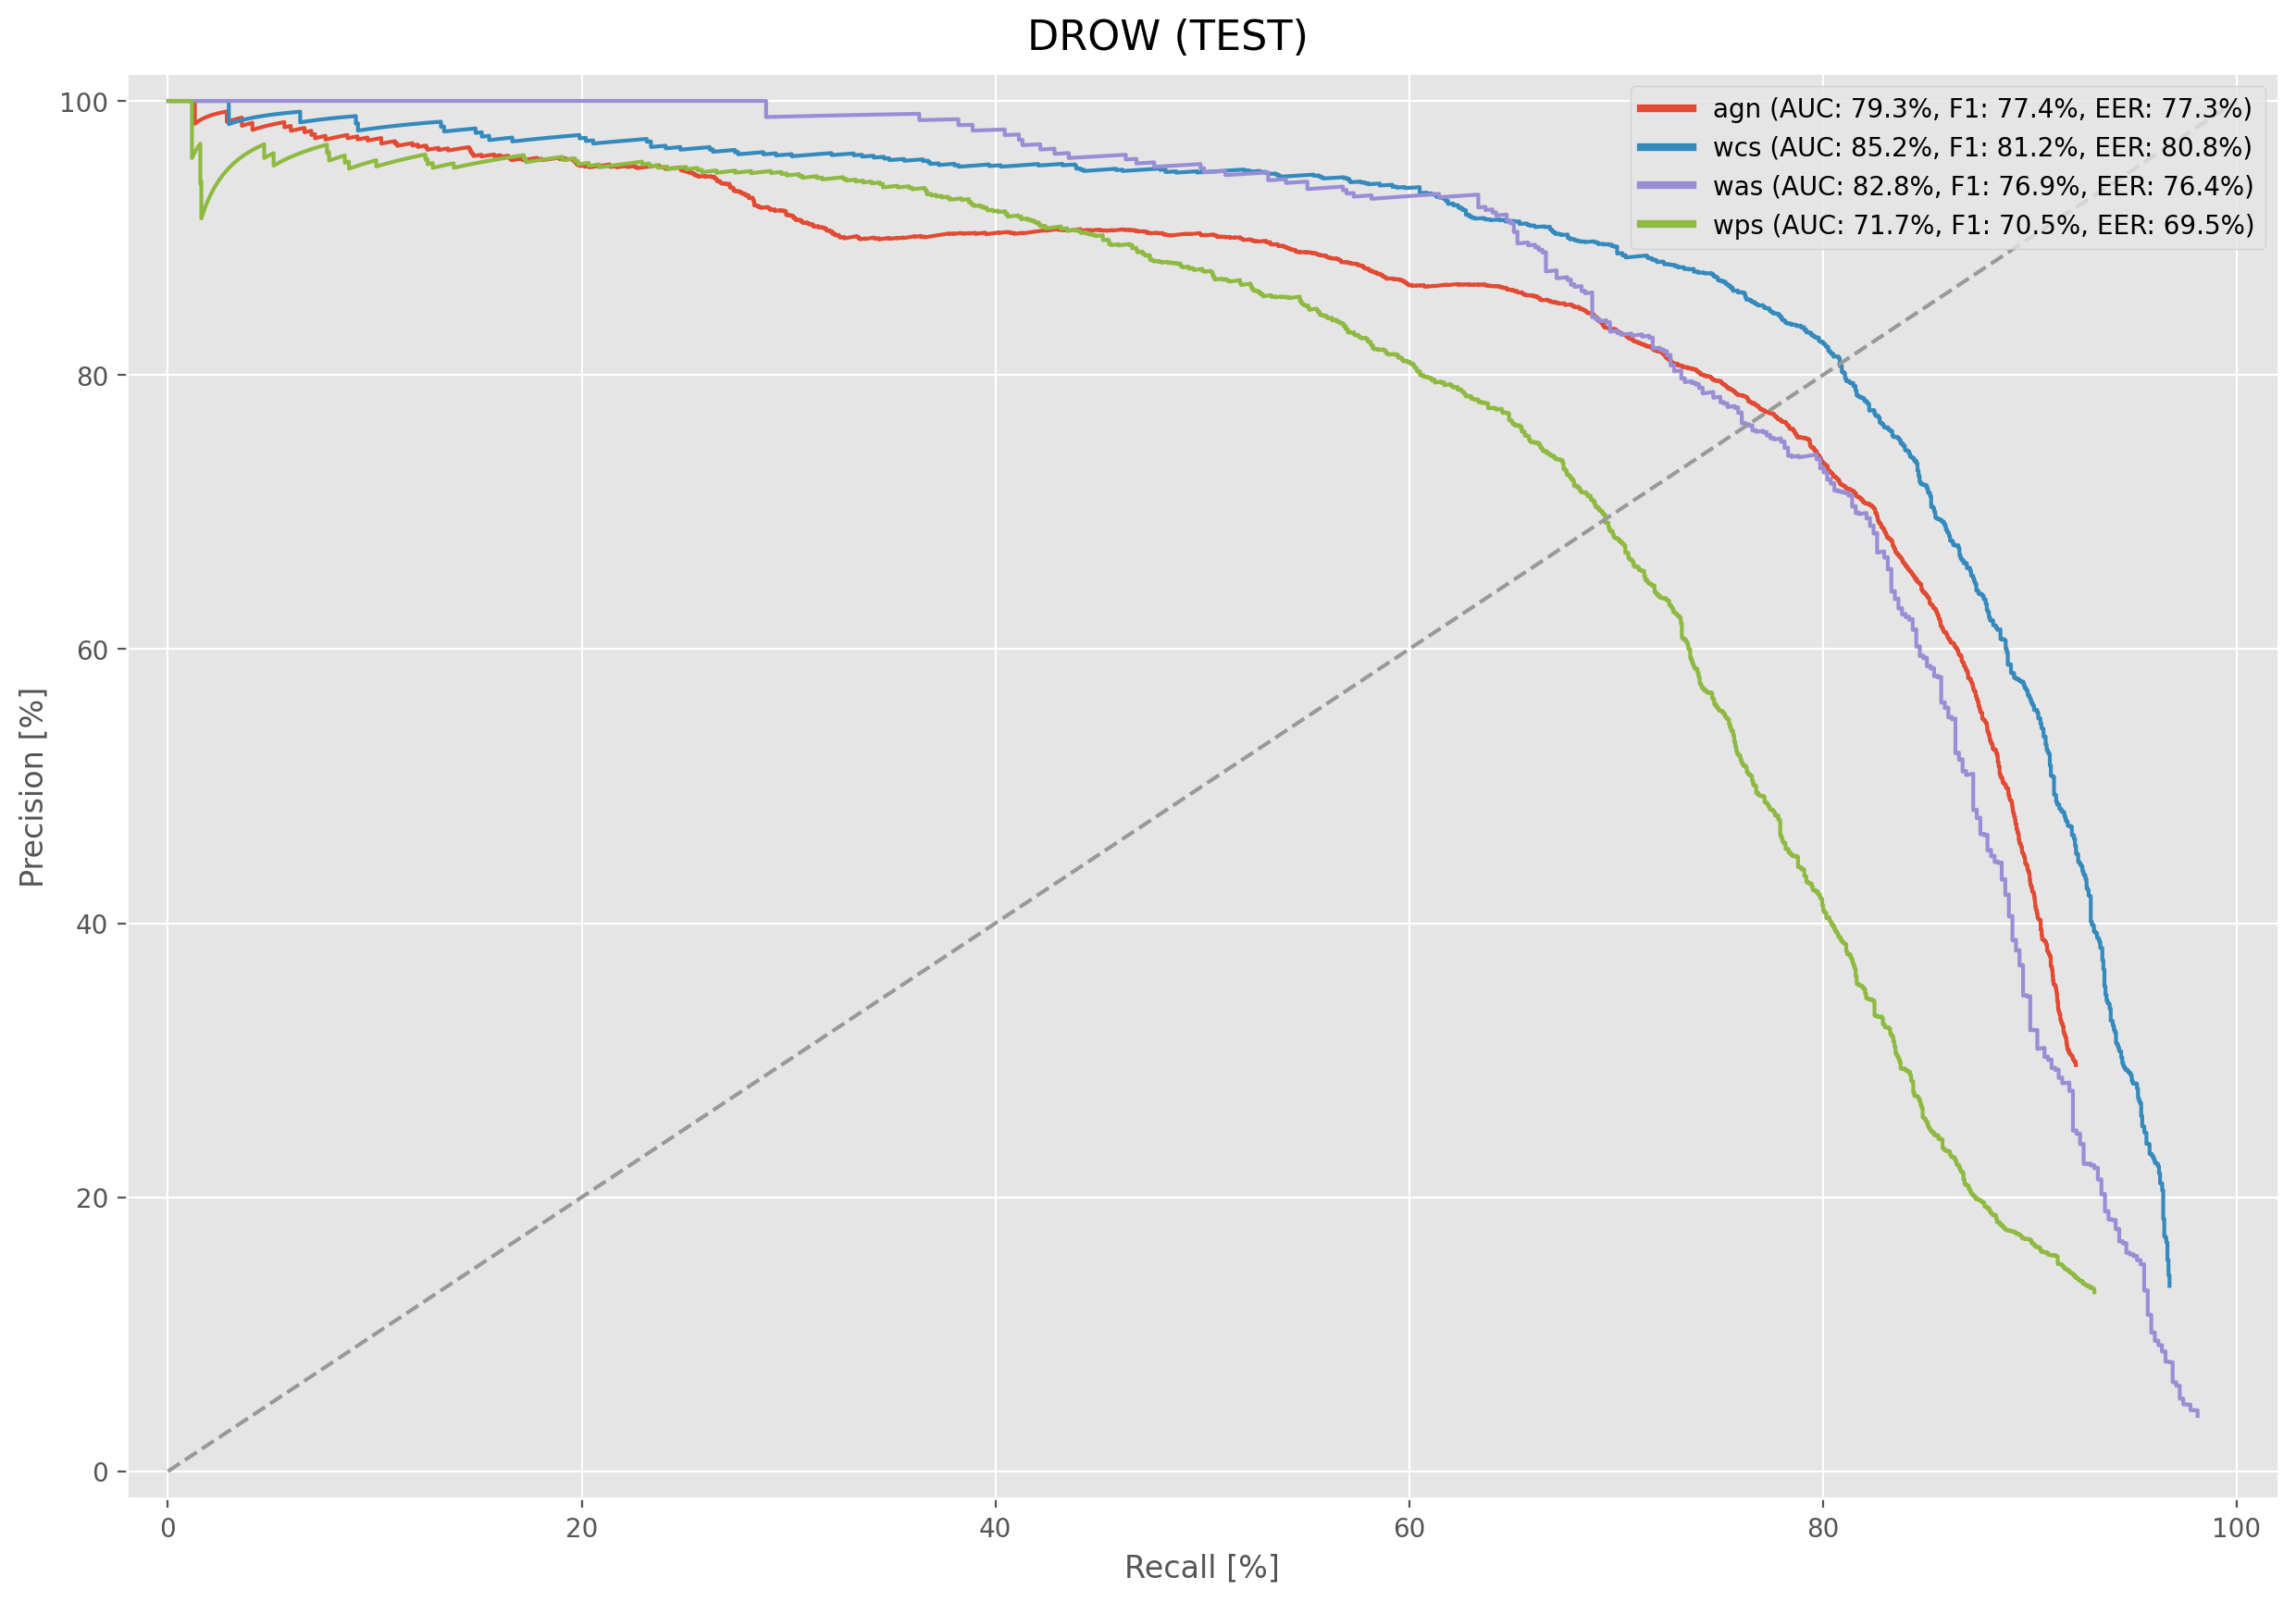
\includegraphics[width=.9\linewidth]{pr_auc_drow}
		\caption{Precision-recall curve of DROW detector}
		\label{fig:pr_auc_drow}
	\end{subfigure}%
	\begin{subfigure}{.5\textwidth}
		\centering
		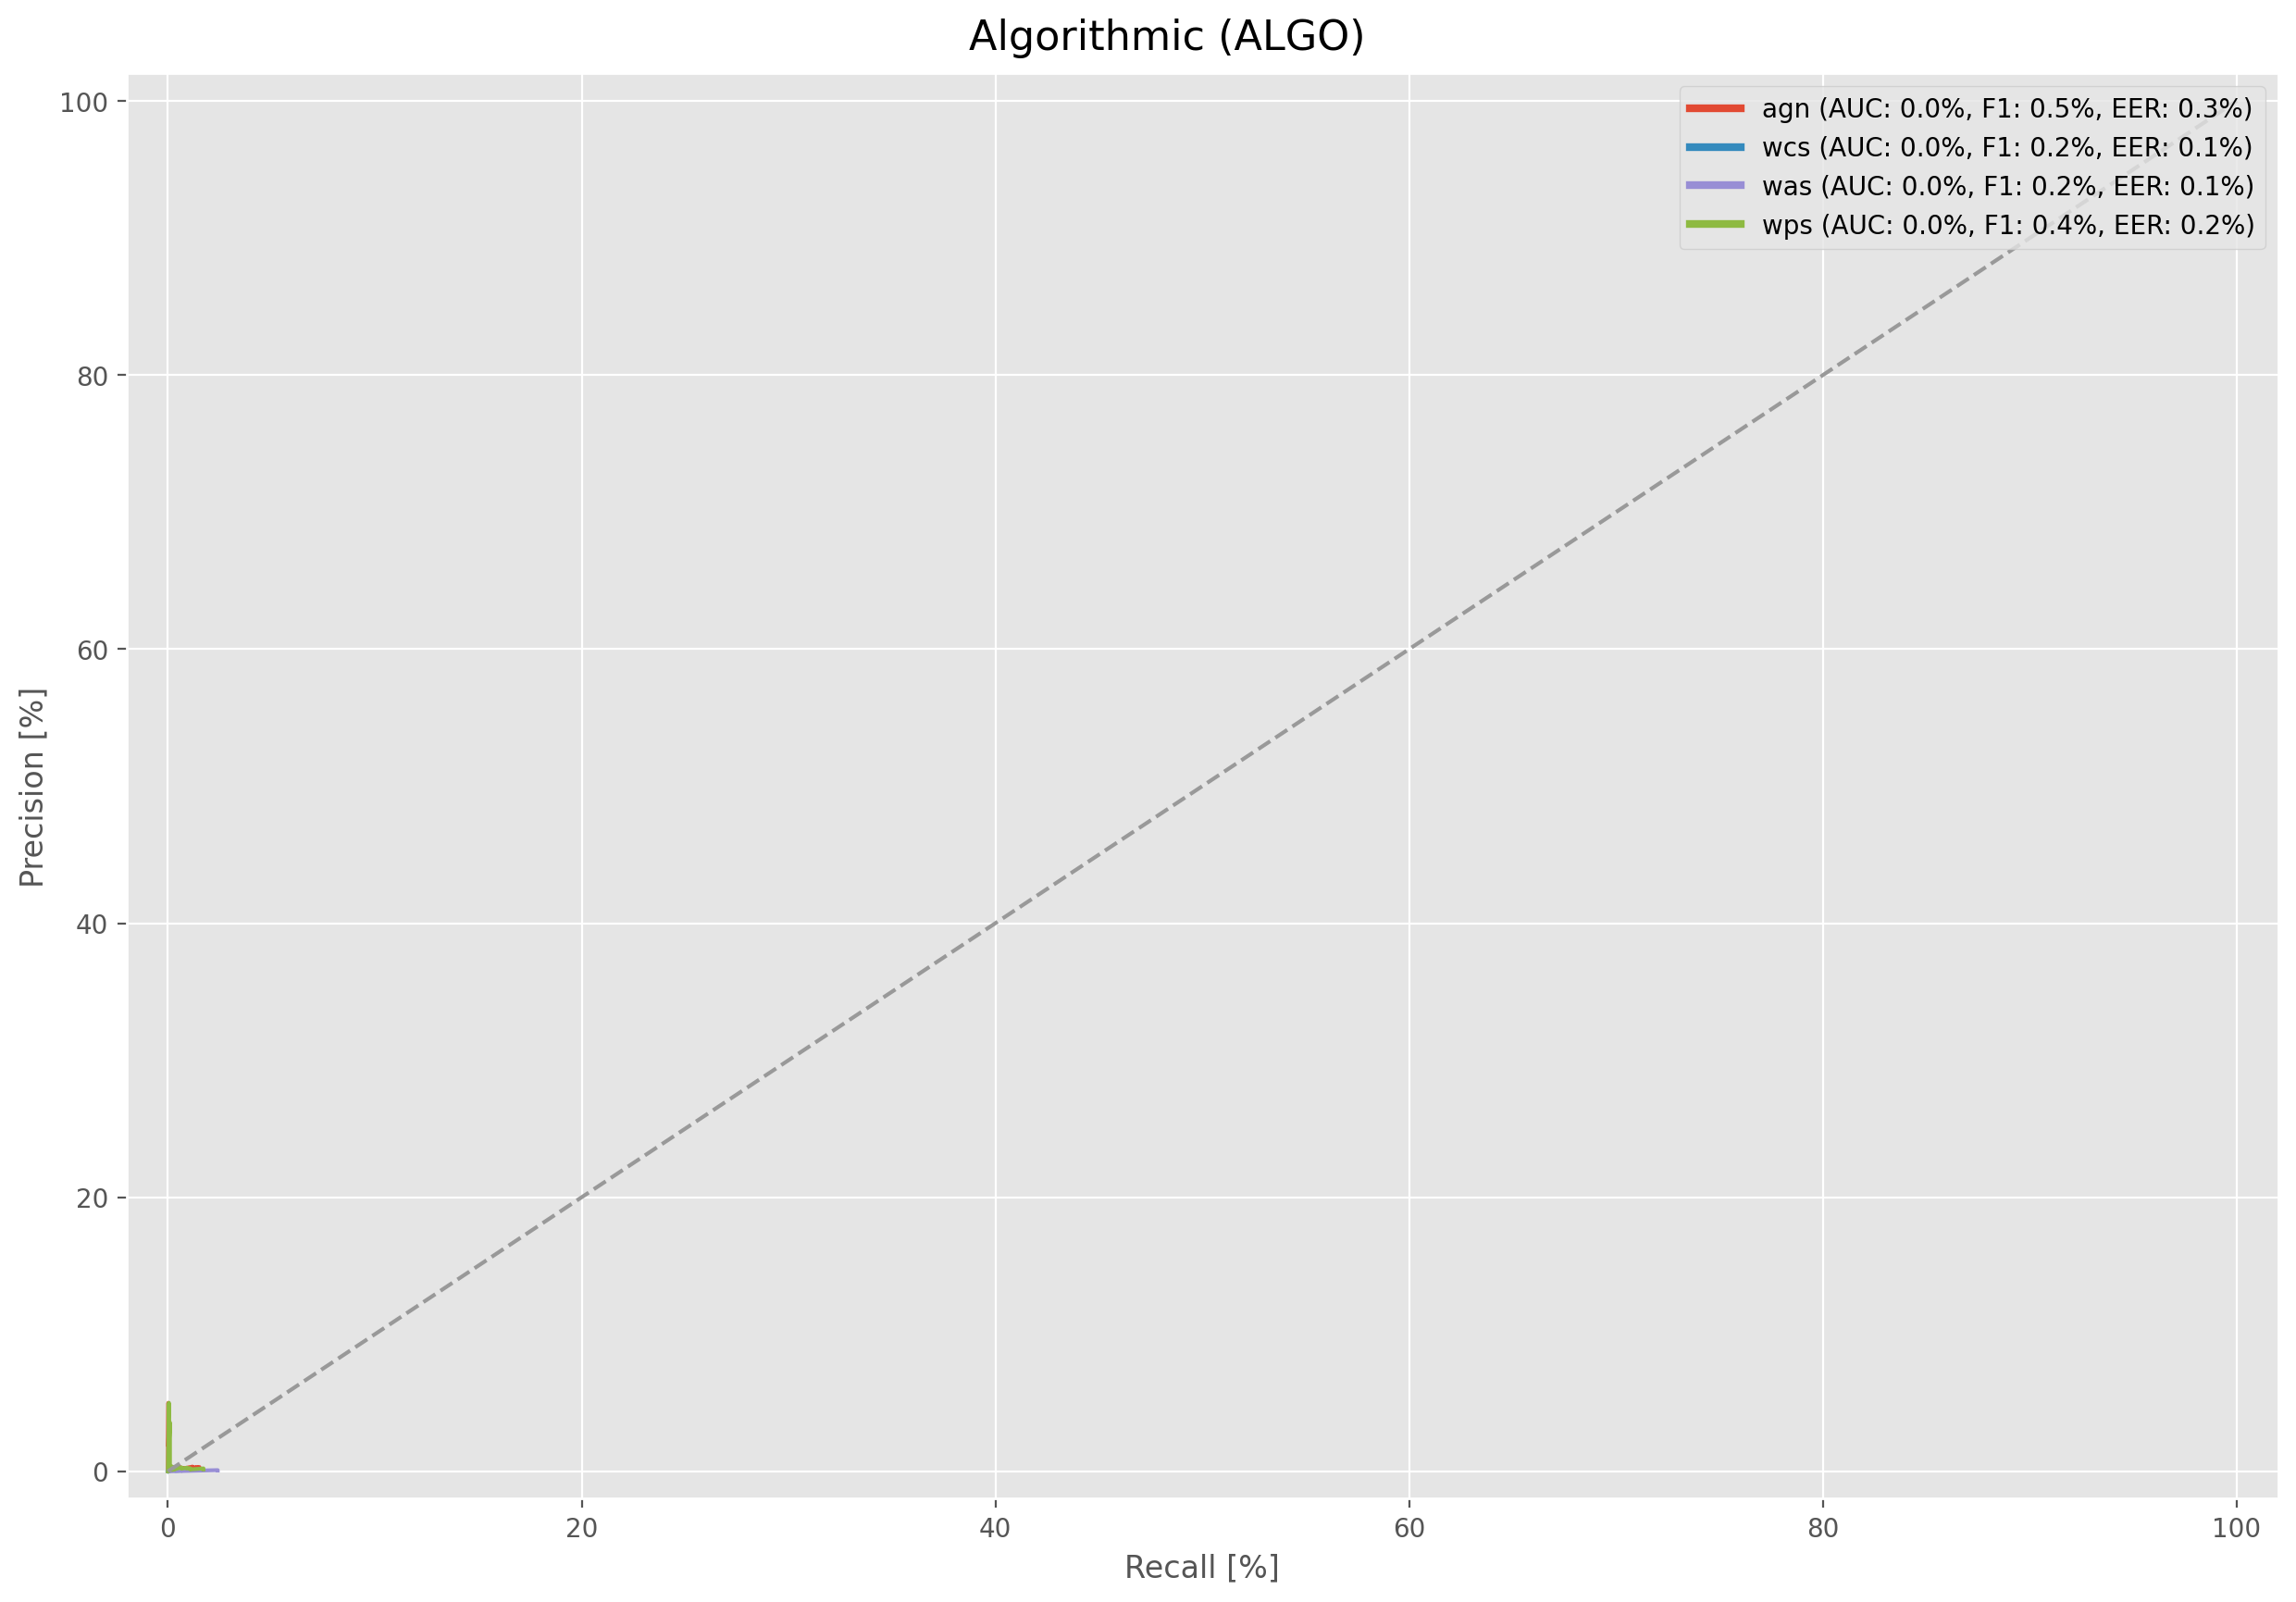
\includegraphics[width=.9\linewidth]{pr_auc_algo}
		\caption{Precision-recall curve of algorithmic detector}
		\label{fig:pr_auc_algo}
	\end{subfigure}
	\caption{Comparison of detectors precision-recall curves}
	\label{fig:pr_auc_comparison}
\end{figure*}

Since the latest ROS 1 version can be installed on Ubuntu Focal Fossa (20.04) only\cite{ros_latest_installation}\cite{ros_latest_package}, a Docker image was created for launching the ROS package on any Linux device.

First, an image with full ROS installation was created.
The image includes all ROS packages installed, \texttt{catkin}\cite{catkin_wiki} workspace created and a running script exporting all required environmental variables.
The image is published on GitHub container registry\cite{FTD_docker_image}.

The other image was build on top of the previous one, it also includes \texttt{follow\_the\_drow} library.
Unfortunately, it couldn't be published because its' size is more than 3Gb, but it can be built and launched locally instead.

A docker compose file was created that sets all environmental variables required for RVIZ graphical output and configures volumes with ROS nodes source code.
This image can also be configured to be used with physical RobAIR by setting special environmental variables.

\section{Results}

Detector comparison was performed on a laptop, using DROW dataset data.
For result storing and visualization, Jupyter notebooks were used.
The notebooks are rendered and available in this paper GitHub repository\cite{FTD_comparison}.

\subsection{Precision-recall comparison}

\begin{figure*}[t]
	\centering
	\begin{subfigure}{.5\textwidth}
		\centering
		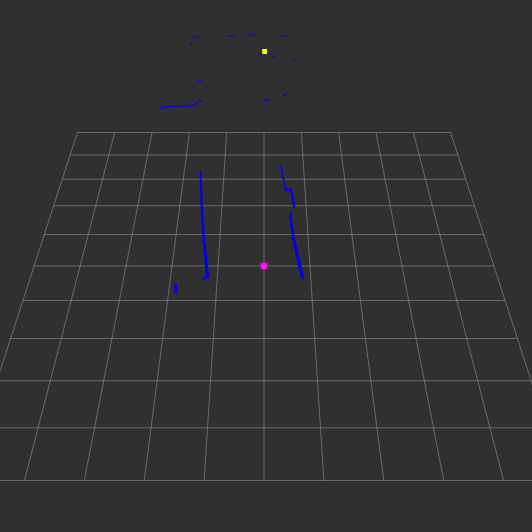
\includegraphics[width=.65\linewidth, height=.65\linewidth]{ftd_false_negative_1}
		\caption{}
		\label{fig:drow_false_negative_1}
	\end{subfigure}%
	\begin{subfigure}{.5\textwidth}
		\centering
		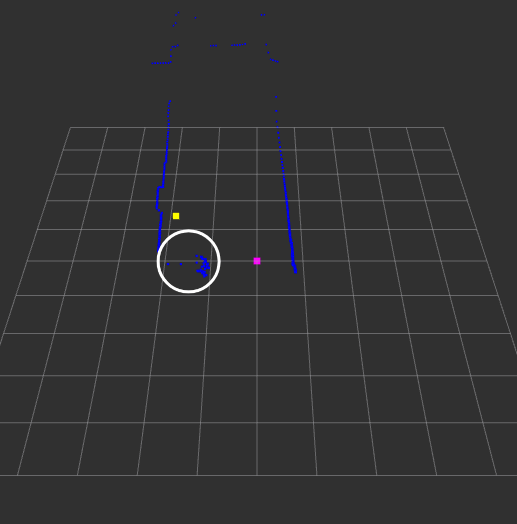
\includegraphics[width=.65\linewidth, height=.65\linewidth]{ftd_false_negative_2}
		\caption{}
		\label{fig:drow_false_negative_2}
	\end{subfigure}
	\parbox[b]{\textwidth}{}
	\begin{subfigure}{.5\textwidth}
		\centering
		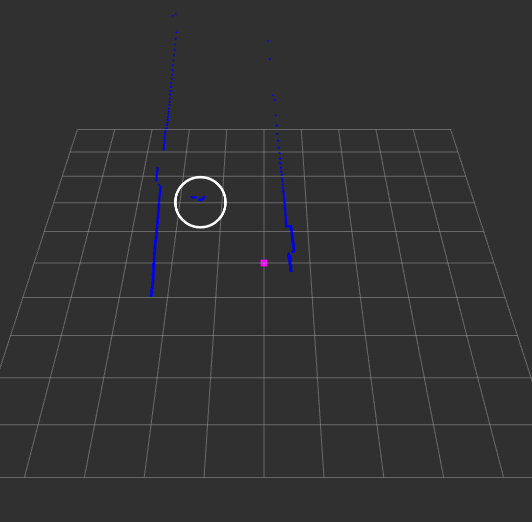
\includegraphics[width=.65\linewidth, height=.65\linewidth]{ftd_false_positive_1}
		\caption{}
		\label{fig:drow_false_positive_1}
	\end{subfigure}%
	\begin{subfigure}{.5\linewidth}
		\centering
		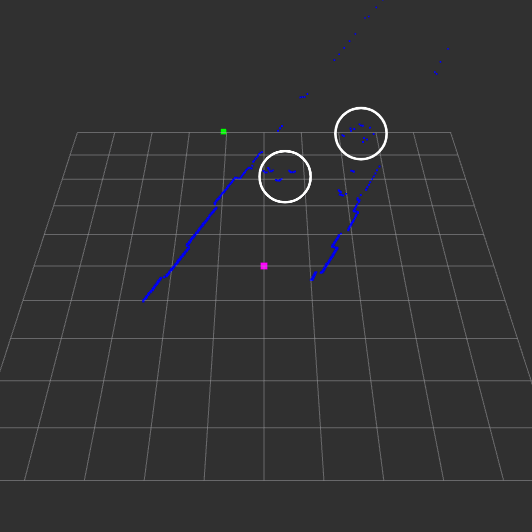
\includegraphics[width=.65\linewidth, height=.65\linewidth]{ftd_false_positive_2}
		\caption{}
		\label{fig:drow_false_positive_2}
	\end{subfigure}
	\caption{DROW dataset incorrect annotation examples}
	\label{fig:drow_annotation_errors}
\end{figure*}

The detection result accuracy was compared by AUC of precision-recall curve\cite{prec_rec_curve}.
Figure \ref{fig:pr_auc_comparison} demonstrates precision-recall curves of the two detectors.
In both cases, DROW dataset annotations were used as "ground truth" for person positions.

The figure \ref{fig:pr_auc_comparison} shows that DROW detector performs significantly better (AUC = 71.1\% for people with visible two legs) than algorithic detector (AUC = 0.0\%).
However, after a closer investigation, it was concluded that the primary reason for the difference was DROW dataset annotations misplacement.

Figure \ref{fig:drow_annotation_errors} shows examples of DROW dataset annotation misplacement.
Pink marker represents the robot, people around it are marked with white circles (manually).
Blue markers represent LiDAR measures, green markers represent person positions predicted by DROW detector and yellow markers represent DROW dataset annotations.

Figures \ref{fig:drow_false_negative_1} and \ref{fig:drow_false_negative_2} show false negative annotation examples, while figures \ref{fig:drow_false_positive_1} and \ref{fig:drow_false_positive_2} show false positive annotation examples.
It has been manually calculated that during the first 3 minutes of DROW dataset recorded data, the annotations match real people positions at most for 20 seconds.

The neural network, trained with this data taken for ground truth can not be expected to find accurate person positions.

\subsection{Execution time comparison}

The detectors execution time was compared by measuring time required by each detector to process a single LiDAR measure.
The following results were obtained:

\begin{itemize}
	\item \textbf{DROW detector} 0.9771 seconds.
	\item \textbf{Algorithmic detector} 0.0001 seconds.
\end{itemize}

RobAIR architecture does not include any graphics processing unit (GPU), so it was decided to run tests on a machine that does not have a GPU either.
The machine CPU is Intel\textregistered{} Core\texttrademark{} i7-3520M CPU @ 2.90GHz and the GPU is integrated in it.

Although the ROS spin rate used for testing was 10Hz (that is still more than the rate used during DROW dataset recording, that is 12.5Hz), that was not enough to run DROW detector each frame.
However, this did not impact other node performance, because ROS nodes run in separate threads and the only visible outcome is that DROW detector markers are updated once per second only.

\section{Conclusion and future work}

Since 2D LiDARs are in many cases preferred to 3D LiDARs and cameras not only because of their price, but also due to lower data processing computational requirements\cite{2D_3D_lidars}, person detection with 2D LiDAR data remains an important task for different kinds of autonomous vehicles.

In this paper, a comparison between two person detectors was made: an heuristic algorithm based detector, relying on some assumptions about human body shape in 2D space, and a neural network based detector, inspired by a popular convolutional neural network VGGnet\cite{vggnet_paper} architecture. 

The two detectors were tested and compared using data from DROW dataset.
The results indicate, that the comparison is not really feasible because of the data in the DROW dataset being annotated incorrectly.
As it can be seen by example provided, in real-world the algorithmic detector performs better (sometimes it detects people).
That, however, does not imply any conclusions about DROW detector architecture - only about the available weights, that were produced by training the neural network on the dataset.
That also does not cover any of the specific cases, that are out of scope of algorithmic detector (wheelchairs, walkers, people in lab coats, etc.).

The \texttt{follow\_the\_drow} pipeline created for detector launching and testing is also considered a contribution of this work.
The pipeline includes:
\begin{itemize}
    \item \texttt{Python} library for testing detectors including bindings for \texttt{C++} code.
    \item ROS package for detector configuration and comparison, that also interoperates with \textbf{Follow me behavior} packages.
    \item Docker image for running latest full ROS 1 distribution on any Linux device in general and \texttt{follow\_the\_drow} ROS package in particular both locally (e.g. for testing purposes) and on a physical robot.
\end{itemize}

Please, consider consulting the paper repository README file\cite{FTD_repo_readme} for information on the ROS package configuration and console commands for testing and comparing the detectors.
Consider consulting special Docker image README manual\cite{FTD_image_readme} for brief explanations of how the published Docker ROS image can be customized and used for other ROS packages running.

As a proposal for incorrect annotation problem solving, an \texttt{Annotator} node was created that allows manual dataset annotation using RVIZ tool graphical user interface.

In order to decrease neural network execution time, several steps might be considered in the future:
\begin{enumerate}
    \item The \texttt{pytorch} library that is used for neural network implementation can be used not only with \texttt{Python}, but also with \texttt{C++}; this might speed up the network execution.
    \item The amount of data processed by the network on a single step can be reduced by using an architecture with recurrent layers instead of processing 5 LiDAR measures at a time; that can also improve the network accuracy (as it is mentioned in the latest DROW article)\cite{DROW_2018}.
    \item Relying on the last LiDAR measure can not only reduce "temporal cutout" calculation time, but also improve the way odometry data is taken into account; for instance, instead of recalculating measure values, odometry difference between frames can be passed directly to neural network.
\end{enumerate}

In general, in laboratory conditions the algorithmic detector performed both faster and more accurate.
However, considering all the specific cases mentioned above that can not be handled by it, DROW (or other convolutional neural network based) person detector, that is trained using a correctly annotated dataset, should be preferred for real world usage.

\clearpage

\bibliographystyle{named}
\bibliography{ijcai11}

\end{document}
